
\chapter{Greffon Statique-Dynamique (StaDy)}
\label{sec:stady}

\chapterintro


Dans ce chapitre nous présentons l'architecture générale du greffon \stady,
notre implémentation de la méthode présentée aux chapitres~\ref{sec:ncd},
\ref{sec:swd} et~\ref{sec:method}, ainsi que certains détails d'implémentation
en partie~\ref{sec:stady-implem}.
En partie~\ref{sec:stady-exp} nous présentons les résultats de nos
expérimentations visant à mesurer la capacité de diagnostic et les performances
de \stady.


\section{Implémentation}
\label{sec:stady-implem}


%\begin{landscape}
\begin{center}
  \begin{figure}
    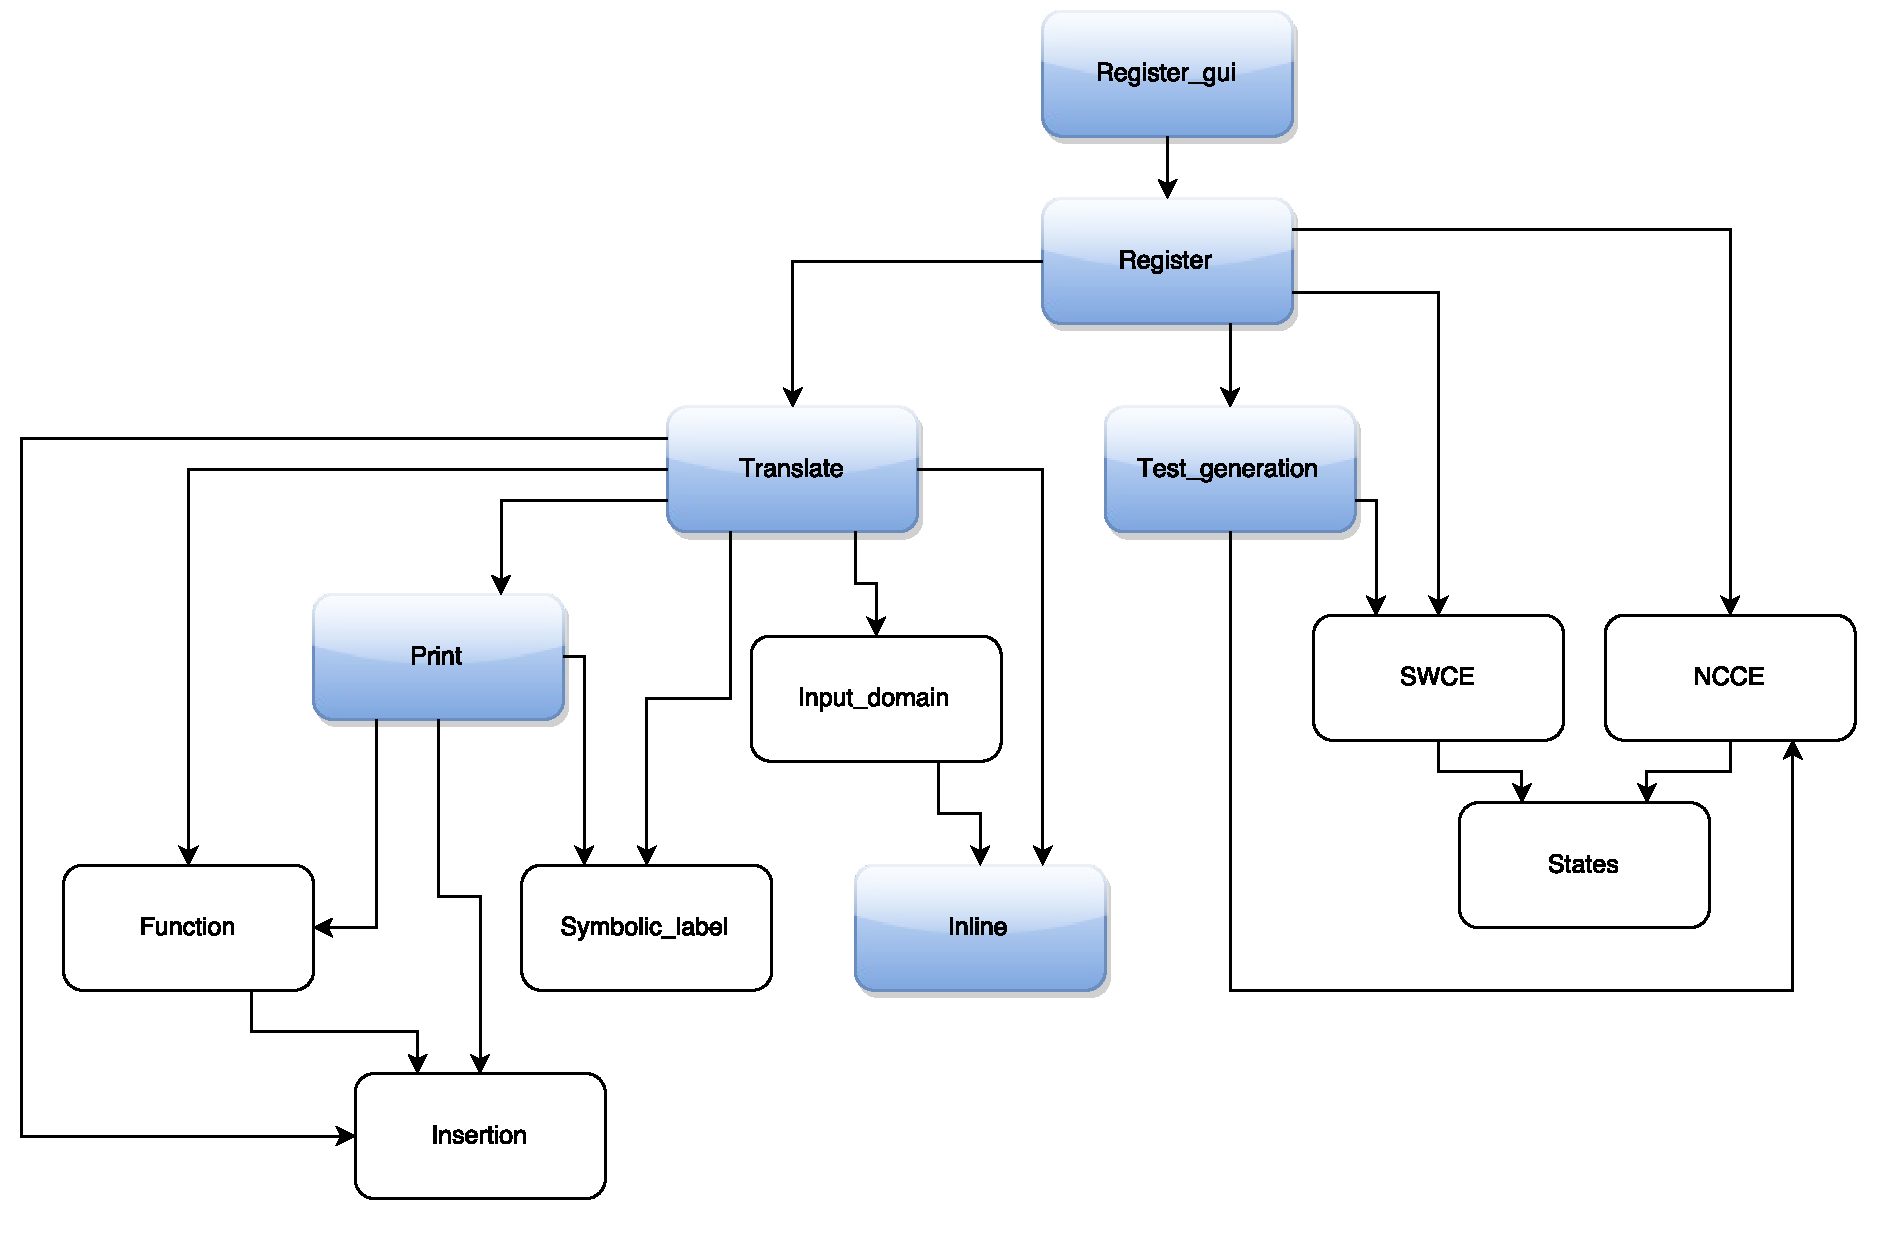
\includegraphics[scale=.5]{figures/stady_architecture.pdf}
    \vspace{-11cm}
    \caption{Architecture de \textsc{StaDy}
      \label{fig:stady-architecture}}
  \end{figure}
\end{center}
%\end{landscape}


\section{Expérimentations}
\label{sec:stady-exp}


\begin{figure}[tb]\scriptsize
  %\vspace{-2mm}
  \begin{center}
    \begin{tabular}{lrr}
      \hline
      example & time (s.) & \# paths \\ \hline
      array-unsafe & 1.299 & 9 \\ \hline
      count-up-down-unsafe & 1.285 & 3 \\ \hline
      eureka-01-unsafe & 1.355 & 48 \\ \hline
      for-bounded-loop1-unsafe & 1.320 & 11 \\ \hline
      insertion-sort-unsafe & 16.530 & 730 \\ \hline
      invert-string-unsafe & 1.359 & 48 \\ \hline
      linear-search-unsafe & 3.624 & 2766 \\ \hline
      matrix-unsafe & 1.367 & 22 \\ \hline
      nec20-unsafe & 1.463 & 1035 \\ \hline
      string-unsafe & 1.362 & 48 \\ \hline
      sum01-bug02-base-unsafe & 1.335 & 26 \\ \hline
      sum01-bug02-unsafe & 1.327 & 36 \\ \hline
      sum01-unsafe & 1.312 & 56 \\ \hline
      sum03-unsafe & 1.291 & 46 \\ \hline
      sum04-unsafe & 1.310 & 22 \\ \hline
      sum-array-unsafe & 1.358 & 14 \\ \hline
      %% trex01-unsafe & 1.561 \\ \hline
      trex03-unsafe & 1.358 & 21 \\ \hline
      sendmail-unsafe & 1.396 & 77 \\ \hline
      vogal-unsafe & 1.349 & 341 \\ \hline
    \end{tabular}
  \end{center}
  \vspace{-3mm}
  \caption{Experiments with \textsc{StaDy}: Bug detection}    
  \label{fig:scam-experiments1}
  \vspace{-3mm}
\end{figure}

\begin{figure}[tb]\scriptsize
  %\vspace{-2mm}
  \begin{center}
    \begin{tabular}{lrrrr}
      \hline
      example & mutants & $\lnot$ equiv. & killed & success rate \\ \hline
      merge-sort & 96  & 92 & 88 & 95.65\% \\ \hline
      merge-arrays & 68 & 63 & 59 & 93.65\% \\ \hline
      quick-sort & 130 & 130 & 130 & 100\% \\ \hline
      binary-search & 40 & 40 & 39 & 97.5\% \\ \hline
      bubble-sort & 52 & 49 & 42 & 85.71\% \\ \hline
      insertion-sort & 39 & 37 & 36 & 97.3\% \\ \hline
      array-safe & 18 & 16 & 15 & 93.75\% \\ \hline
      bubble-sort-safe & 64 & 58 & 55 & 94.83\% \\ \hline
      count-up-down-safe & 14 & 13 & 13 & 100\% \\ \hline
      eureka-01-safe & 60 & 60 & 60 & 100\% \\ \hline
      eureka-05-safe & 36 & 36 & 36 & 100\% \\ \hline
      insertion-sort-safe & 43 & 41 & 40 & 97.56\% \\ \hline
      invert-string-safe & 47 & 47 & 47 & 100\% \\ \hline
      linear-search-safe & 19 & 17 & 16 & 94.12\% \\ \hline
      matrix-safe & 30 & 27 & 25 & 92.59\% \\ \hline
      nc40-safe & 20 & 20 & 20 & 100\% \\ \hline
      nec40-safe & 20 & 20 & 20 & 100\% \\ \hline
      string-safe & 65 & 65 & 65 & 100\% \\ \hline
      sum01-safe & 14 & 14 & 13 & 92.86\% \\ \hline
      sum02-safe & 14 & 14 & 11 & 78.57\% \\ \hline
      sum03-safe & 10 & 10 & 10 & 100\% \\ \hline
      sum04-safe & 14 & 14 & 10 & 71.43\% \\ \hline
      sum-array-safe & 17 & 17 & 15 & 88.24\% \\ \hline
      trex03-safe & 56 & 56 & 56 & 100\% \\ \hline
      sendmail-safe & 31 & 31 & 31 & 100\% \\ \hline
      vogal-safe & 71 & 68 & 67 & 98.53\% \\ \hline
      \textbf{Total} & 1088 & 1054 & 1019 & \textbf{96.68\%} \\ \hline
    \end{tabular}
  \end{center}
  \vspace{-3mm}
  \caption{Experiments with \textsc{StaDy}: Mutation testing}
  \label{fig:scam-experiments2}
  \vspace{-3mm}
\end{figure}

The current implementation of  
\textsc{StaDy} supports a significant subset of \eacsl including
assertions, pre- and postconditions, loop invaliants and variants,
quantifications, logic functions, integral and pointer types, and
basic pointer operations. Pointer validity is currenty supported
only for input arrays and pointers.
\textsc{StaDy} currently  does not support 
\lstinline{assigns} clauses, \lstinline{\at} terms, 
real numbers, as well as advanced memory-related constructs
(e.g. \lstinline{\offset}), complex pointer
arithmetics such as \lstinline'p1-p2' or \lstinline'*(p-i)' and dynamic memory allocation  
due to the limitations of the underlying test generator. 
%Annotations involving reals
%($\mathbb{R}$) are not supported either.

To evaluate the efficiency of \textsc{StaDy} 
%to find counter-examples 
in a combined verification approach
(cf Sec. \ref{sec:motivations}),
we applied it on safe and unsafe programs from the TACAS 2014
Software Verification Competition%
\footnote{\url{https://svn.sosy-lab.org/software/sv-benchmarks/trunk/c/loops}}
%(selected from the subdirectory {\em loops})
%to evaluate its efficiency. 
First, we 
%tracked down bugs in faulty programs.
%We 
executed \textsc{StaDy} on 20 faulty programs that  handle arrays
with loops. The properties to invalidate originally 
expressed as C assertions, were manually rewritten in \textsc{E-ACSL}.
Adequate \textsc{E-ACSL} preconditions were also added. The programs
containing infinite loops and reachability properties to invalidate are not
handled by  \textsc{StaDy} due to the necessity to execute the program in
\textsc{Path\-Crawler}.
\textsc{Sta\-Dy}
 detected failures of all faulty properties in each considered program. 
Fig.~\ref{fig:scam-experiments1} illustrates the time taken to
invalidate the properties including all the steps of \textsc{Sta\-Dy}:
instrumentation from the \textsc{E-ACSL} specifications and test generation in
\textsc{PathCrawler}, and the number of explored paths.

Secondly, we used  mutation testing to evaluate the ability of \textsc{StaDy} to
find bugs in unsafe programs. % automatically generated from safe programs.
We selected 20 safe programs of the same benchmark, and 6
additional safe programs from our own benchmarks. All of them were annotated in
\textsc{E-ACSL}. They contain preconditions, postconditions, assertions,
memory-related properties, loop variants and invariants. We used mutation testing
on these safe programs to generate modified programs (\emph{mutants}) and see if
\textsc{StaDy} is able to \emph{kill} 
(i.e. to find errors in) these mutants. The
mutations performed on the source code mimic usual programming errors. They
include modifications of numerical and/or pointer arithmetic operators,
comparison operators, condition negation and logical operators ({\em and} and
{\em or}). Fig.~\ref{fig:scam-experiments2} gives the 
numbers of all and erroneous mutants, as well as 
the number and proportion of erroneous mutants killed by \textsc{StaDy}. 
\textsc{StaDy} showed 
an average success rate of 96.68\%, going up to 100\% on many examples.
The missing percents are mostly due to 
%the incompleteness of the specifications
%in some programs, explained by 
a currently incomplete support of \textsc{E-ACSL} features
by the underlying test generation tool.


%%%%%%%%%%%%%%%%%%%%%%%%%%%%%%%%%%%%%%%%%%%%%%%%%%%%%%%%%%%%

\begin{figure*}[bt]
  \tiny
\mbox{}\hspace{-20mm}
  \begin{center}
  \begin{tabular}{r|c|c|c|c|c|c|c|c|c|c|c|c|c|c|c}
    &&\multicolumn{3}{c|}{Proof}&\multicolumn{4}{c|}{\NCD}
    &\multicolumn{4}{c|}{\CWD}&\multicolumn{2}{c|}{$\NCD+\CWD$}&\\
    \hline
    \input{full_exp_latex_IEEE.csv}
  \end{tabular}
\end{center}
  \caption{Detailed experiments of proof failure diagnosis for mutants with \stady}
  \vspace{-.5cm}
  \label{tab:exp}
\end{figure*}


\textbf{Implementation.}
The proposed method for diagnosis of proof failures 
% detecting  non-compliances and contract weaknesses
%described in Sec.~\ref{sec:global-method} 
has been implemented as a \framac plugin, named \stady.
It relies on other plugins: \Wp~\citeframac for deductive
verification and \pathcrawler~\citepathcrawler for structural test generation.
\stady currently supports a significant subset of the \eacsl specification
language, including 
\lstinline'requires', \lstinline'ensures', 
\lstinline'behavior', \lstinline'assumes', 
\lstinline'loop invariant', \lstinline'loop variant' and
\lstinline'assert' clauses.
Quantified predicates
\lstinline[style=c]'\exists' and \lstinline[style=c]'\forall' and builtin terms
as \lstinline'\sum' or \lstinline'\numof' are translated as loops. 
Logic functions and named predicates are treated by inlining.
The \lstinline'\old' constructs are treated by saving the initial
values of formal parameters and global variables at the beginning of the
function. 
Validity checks of pointers are
partially supported due to the current limitation of the underlying test
generator: we can only check the validity of input pointers and global arrays.
The \lstinline'assigns' clauses are only taken into consideration during the
\CWD phase: we do not aim to find what is missing in the \lstinline'assigns'
clause (\NCD) because provers usually give sufficiently good feedback about it,
but we want to find what is unnecessary and could be removed from an
\lstinline'assigns' clause (\CWD).
Inductive predicates, recursive functions and floating-point numbers are
currently not supported and are part of our future work.

\textbf{The research questions} we address in our experiments are the following.

\vspace{-2mm}
\begin{itemize}
\item[\textbf{RQ1}]
Is \stady able to precisely diagnose most proof failures in C programs?
\item[\textbf{RQ2}]
What are the benefits of the \CWD extension (in particular, with respect to
\NCD)?
\item[\textbf{RQ3}]
Is \stady able to generate  \NCCE{}s or \CWCE{}s even with a partial testing coverage?
\item[\textbf{RQ4}]
Is \stady's execution time comparable to the time of an automatic proof?
\end{itemize}
\vspace{-2mm}



\textbf{Experimental protocol.} 
The evaluation used 20 annotated programs from \cite{ACSLbyExample},
whose size varies from 35 to 100 lines of annotated C code.
%binary\_search, binary\_search2, lower\_bound, upper\_bound, max\_element,
%max\_element2, max\_seq, min\_element, copy, fill, iota, replace\_copy,
%reverse\_copy, adjacent\_find, equal, equal2, equal3, find, find2 and mismatch.
These programs manipulate arrays, they are fully specified in \acsl and their
specification expresses non-trivial properties of C arrays. 
To evaluate the method
presented in Sec.~\ref{sec:global-method} and its implementation, we apply \stady on systematically
generated altered  versions (or \emph{mutants}) of correct C programs.
%We apply the method presented in Sec.~\ref{sec:method} and measure the
%efficiency of the classification performed by \stady.
%Each utants are generated for each considered program 
Each mutant program is obtained by performing a single modification (or \emph{mutation}) on the
initial program.
The mutations include: a binary operator modification in the code or in the
specification, a condition negation in the code, a relation modification in the
specification, a predicate negation in the specification, a partial loop invariant or
postcondition deletion in the specification.
In this study, we do not mutate the precondition of the function under verification, 
and restrict possible mutations on binary operators to avoid creating absurd
expressions, in particular for pointer arithmetics.


The first step tries to prove each mutant using \Wp. 
%(with a timeout high enough \commentNK{preciser}).
The proved mutants respect the specification and are classified as correct. 
% are equivalent to the original program. % NK: Not sure!
Second, we apply the \NCD method on the remaining mutants.
It classifies proof failures for some mutants as non-compliances, indicates the failing annotation and an \NCCE.
The third step applies the \CWD method on remaining mutants,
classifies some of them as subcontract weaknesses, indicates the weak subcontract and a \CWCE.
If no counter-example has been found by the \CWD, the mutant remains 
unclassified. % (the \textsf{?} column).
%\commentNK{preciser timeouts here}
The results are displayed in Fig.~\ref{tab:exp}.
The columns 
%of  Fig.~\ref{tab:exp}  
present the number of generated mutants, and the results of each of the three
steps: the number (\#) and ratio (\%) of classified mutants,
maximal and average execution time (put on two lines) of the step
over classified mutants ($t^\text{\ok}$ or $t^\text{\ko}$) and over non-classified
mutants ($t^\text{?}$) at this step.
The ratios are computed with respect to unclassified mutants after the previous step.
The $\NCD+\CWD$ columns sum up selected results after both $\NCD$ and $\CWD$ steps:
the average and maximal time ($t$) are shown globally over all mutants.
The time is computed until the proof is finished or until the first counter-example is generated.
The final number of remaining unclassified mutants (\#?) is given in the last column.


\textbf{Experimental results.}
%\textbf{RQ1.}
%Regarding RQ1,
For the 20 considered programs, 928 mutants have been generated. 80 of them 
%are equivalent and 
have been proved by \Wp.
Among the 848 unproven mutants, \NCD has detected a non-compliance
induced by the mutation in 776 mutants (91.5\%),
leaving 72 unclassified.
Among them, \CWD has been able to exhibit a counter-example (either a \NCCE or a
\CWCE)
%, the confirmation step is not automatized yet) %NK: to be done for the final version
%for the contract impacted by
%the mutation in
for 48 of them (66.7\%), finally leaving 24 programs unclassified.
They can be either equivalent mutants that were not proved
by \Wp due to a prover incapacity, or mutants coming from a mutation 
in an unsupported annotation being undetectable by the
current version, or incorrect mutants for which testing was incomplete due to a timeout.
Regarding \textbf{RQ1}, \stady has found a precise reason
of the proof failures  and produced a counter-example 
in 824 of the 848 unproven mutants, 
i.e. classifying 97.2\%.
Exploring the benefits of detecting a prover incapacity may often require to manually reduce
the input domain, to try additional lemmas or interactive proof, so it   
was not sufficiently investigated in this study 
(and would probably require another, non mutational approach).

%\textbf{RQ2.}
Regarding \textbf{RQ2}, 
\NCD alone diagnosed 776 of 848 unproven mutants (91.5\%).
\CWD diagnosed 48 of the 72 remaining  mutants (66.7\%)
bringing a significant complementary contribution 
to a better understanding of reasons of many proof failures.
%The combined efforts of \NCD and \CWD classified 824 of 848 non-equivalent mutants
%(97.2\%), so \CWD permitted to add roughly 6\% to the fault detection efficiency
%of \NCD.

%\textbf{RQ3.}
In our experiments,
each prover can try to prove each verification condition 
%proof obligation 
during at most 40 seconds.
We also set a timeout for any test generation session
to 5 seconds, i.e. one session for the \NCD step, and 
several sessions for \CWD steps.
We also limit the depth of explored program paths with the 
{\em k-path} criterion (cf. Sec. \ref{sec:framac})
%With this option, the test generator only considers paths with at most
%$k$ consecutive iterations of each loop. 
setting $k = 4$.
Both the session timeout and the {\em k-path} heavily limit the testing coverage
but \stady still detects 97.2\% of faults in the generated programs.
That addresses \textbf{RQ3} and demonstrates that the proposed method can efficiently 
classify proof failures and generate counter-examples
even with a partial testing coverage and can therefore 
be used for programs where the 
total number of paths cannot be limited
(e.g. by the \lstinline{typically} clause).

%\textbf{Time of analysis.}
Concerning \textbf{RQ4},
on the considered programs \Wp needs on average 2.6 sec. per mutant (at most 4.4 sec.) to
prove a program, and spends 13.0 sec. on average (at most 61.3 sec.) when the
proof fails.
The total execution time of \stady is comparable: it needs on average 2.7 sec.  per unproven mutant 
(at most 19.9 sec.).
%More precisely, the \NCD step needed 2.4 sec. on average (at most 9.4 sec.) to
%detect a non-compliance, and on average 2.5 sec. (at most 8.3 sec.) when it is
%non conclusive.
%The \CWD step needed 2.4 sec. on average (at most 6.4 sec.) to
%detect a contract weakness, and on average 6.3 sec. (at most 11.6 sec.) when it
%is non conclusive.

\textbf{Summary.}
The experiments show that the proposed method can automatically classify a significant number
of proof failures within an analysis time comparable to the time of an automatic proof
and for programs for which only a partial testing coverage is possible.
The \CWD technique offers an efficient complement to \NCD for a more 
complete and more precise diagnosis of proof failures.

\textbf{Threats to validity.}
As it is often the case in software verification studies, one major threat is
related to the 
representativeness of results, i.e. their \textit{external validity}.
In our case, due to the nature of the problem,
we are restricted to realistic annotated programs
that cannot be generated automatically 
or extracted from existing databases of unspecified code.
Therefore, to reduce this threat, we used programs from an \textit{independent}
benchmark \cite{ACSLbyExample} created in order to illustrate
on different examples the usage of the \acsl specification 
language for deductive verification with \framac.


%Though, the primary contribution of this article is to propose 
%a novel classification of proof failures and techniques
%for their classification.

\textit{Scalability} of the results is another threat
since we do not demonstrate their validity for functions of larger programs. 
%While this is an important issue we plan to address in the near future, 
%However,  
Because of the modular reasoning of deductive verification,
it can be argued that the proposed technique should only be applied on a unit level,
separately for each function, since the verification engineer proves a program  in this way.
Indeed, in the current practice of deductive verification, it does not make sense to analyze
proof failures for the whole module or application at the same time.

The main scalability concern is thus related to the usage of structural test generation 
that can often time out without achieving a full coverage.
To address this issue, we have specifically investigated the impact of a partial test coverage
on the effectiveness of the method (cf. \textbf{RQ3} above) and proposed
a convenient way to reduce the input domain (using \lstinline{typically} clause, 
an extension of \acsl).

Other threats can be due to the used measurements, i.e. \textit{construct validity}.
To reduce this threat, we used a careful measurement of 
results (including analysis time for each step and 
each mutant, their mean and maximal values, 
separately computed for classified and unclassified proof failures).
One concern is producing realistic situations in which 
the verification engineer can need help in the analysis of proof failures.
While the first users of \stady have appreciated its feedback, % \cite{ggp15},
we have not yet had the opportunity to organize a fair evaluation with a 
representative group of users. 
Thus we have performed an extended set of experiments using simulation of 
errors by mutations as an alternative in the meanwhile. 
We have chosen a large subset of mutation operators (mutation in the code,
mutation in an annotation, deletion of an annotation) that model 
frequent problematic situations 
(incorrect code or annotations, incomplete specification)
leading to proof failures.
This approach looks suitable for non-compliance and subcontract weaknesses, and
certainly less suitable for the more subtle prover incapacity cases.
The results should be later confirmed by a representative user study.


\section*{Conclusion du chapitre}


Dans ce chapitre, nous avons présenté l'architecture du greffon \stady, notre
implémentation de la méthode présentée aux chapitres~\ref{sec:ncd},
\ref{sec:swd} et~\ref{sec:method}.
Nous avons également présenté les résultats de nos expérimentations évaluant
la capacité de diagnostic et les performances de \stady.
